\newcommand{\mess}[3] {
\begin{figure}[htbp]
	\centering
	\includegraphics[width=0.8\textwidth]{#1}
	\caption{#2}
	\label{#3}
\end{figure} }
\newcommand{\refabb}[1]{(siehe Abb. \ref{#1})}
\chapter{Durchführung}

\section{Solarzelle}
Als Solarzelle kommt eine Anordnung von 6 Einzelzellen zum Einsatz. Zuerst messen wir die Leerlaufspannung und den Kurzschlussstrom der Anlage bei verschiedenen Beleuchtungsstärken.
\begin{center}
\begin{tabular}{ |  l  c  c  c | }
\hline
	& Tisch	& Fenster & unter Tisch \\ \hline	
Leerlaufspannung & $\SI{0,665}{\volt}$	& $\SI{1,979}{\volt}$	& $\SI{0,173}{\volt}$ \\ 
Kurzschlussstrom & $\SI{0,95}{\milli \ampere}$	& $\SI{9,89}{\milli \ampere}$	& $\SI{0,18}{\milli \ampere}$ \\ 
\hline
\end{tabular}
\end{center}

Wir messen nun die I/U-Kennlinie der Zellen im Dunklen \refabb{a2}.
Aus dieser Kennlinie erzeugen wir die P/I-Kennlinie. Im Dunklen ist die Leistung hier positiv, die Zellen wirken also als Verbraucher \refabb{a2pi}. 
\mess{mess/aufg2.pdf}{Dunkel I/U-Kennlinie der Solarzellen}{a2}
\mess{mess/aufg2_pi.pdf}{Dunkel P/I-Kennlinie der Solarzellen: Zellen wirken als Verbraucher}{a2pi}

Nun messen wir die I/U-Kennlinie bei beleuchteter Zelle. Dazu schalten wir verschiedene Lastwiderstände vor \refabb{a3}. 
\mess{mess/aufg3_iu.pdf}{I/U-Kennlinie der Solarzellen}{a3}
Aus dieser erzeugen wir wiederum die P/I-Kennlinie \refabb{a3pi}
\mess{mess/aufg3_pi.pdf}{P/I-Kennlinie der Solarzellen}{a3pi} 
Gefittet wurde die I/U-Kennlinie mit dem Zusammenhang:
\[
I(U) = y_0 + I_0 \, e^{\frac{U}{U_0}}
\]
Aus dem Fit ergeben sich die Werte:
\begin{align*}
	y_0 &= \SI{-9.48}{\milli \ampere}\\
	I_0 &= \SI{0.28}{\milli \ampere}\\
	U_0 &= \SI{0.55}{\volt}
\end{align*}
Für $U=0$ ergibt sich der Kurzschlussstrom $I_K$ und für $I=0$ die Leerlaufspannung $U_L$.
\begin{align*}
	I_K &= I(0) = y_0 + I_0 = \SI{-9,2}{\milli \ampere} \\
	U_L &= U(0) \\
	&\Rightarrow U(I) = U_0 \ln \left( \frac{I-y_0}{I_0} \right) \\
	U_L &= U_0 \ln \left( -\frac{y_0}{I_0} \right) = \SI{1,9}{\volt}
\end{align*}

Verunreinigungen und Kristallfehler and der Grenzfläche der p-n leitenden Schicht verursachen Widerstände die sich im realen nicht auf 0 (Reihe) und unendlich (Parallel) setzen lassen.
Dabei wäre der Füllfaktor bei 1 und der MPP folglich am besten.
Um diese Widerstände zu bestimmen nutzt man die Kennlinie des Bauteils.
Diese Widerstände entsprechen den Steigungen der Kennlinie nahe den Achsen, also der Steigung des Graphen bei Leerlaufspannung und Kurzschlussstrom.
Wir erhalten daraus die Werte:
\[
R_s=R(0)=-\frac{U_0}{y_0}=\SI{58}{\ohm}, \qquad
R_p=R(I_K)=\frac{U_0}{I_0}=\SI{2,0}{\kilo \ohm}
\]
Diese Werte sind in etwa realistisch für unsere Bedingungen. Die Tendenz, dass der Parallelwiderstand hoch ist und der Reihenwiderstand gering ist, ist gegeben. Die Werte wurden am Fenster aufgenommen.

Mit $P=UI$ stellen wir nun die Fit-Funktion für das P/I-Diagramm auf, um den Maximum Power Point zu bestimmen.
\[
	P(I)=U(I) \cdot I=U_0 \cdot \ln \left( \frac{I-y_0}{I_0} \right) \cdot I
\]
Aus dem Graphen erhalten wir $P_{MPP}= \SI{-8,5}{\milli \watt}$ und $I_{MPP} = \SI{-6,5}{\milli \ampere}$.
Daraus ergibt sich für Spannung und Widerstand
\begin{align*}
	U_{MPP} &= U(I_{MPP}) = \SI{1,3}{\volt} \\
	R_{MPP} &= \frac{U_{MPP}}{I_{MPP}} = \SI{0,2}{\kilo \ohm}
\end{align*}

Hieraus lässt sich auch der Füllfaktor bestimmen.
\[
	f= \frac{U_{MPP} \cdot I_{MPP}}{U_L \cdot I_L} = 0.49
\]
Der Literaturwert für amorphe Solarzellen liegt bei 0.5-0.7. Durch das Durchführen des Versuches ohne direkte Sonneneinstrahlung geht der errechnete Wert in Ordnung.

Zuletzt untersuchen wir den Zusammenhang zwischen Leistung und beleuchteter Fläche. Hierzu bedecken wir schrittweise ein halbes Solarpanel pro Messung. Aus dem Plot \refabb{a4} ist der quadratische Zusammenhang zu erkennen. Dies ist das Resultat der Mischung aus Reihen- und Parallelschaltungen der einzelnen Solarmodule. 
\mess{mess/aufg4.pdf}{Zusammenhang zwischen Leistung und beleuchteter Fläche}{a4}

\section{Elektrolyseur}

\begin{figure}[htbp]
	\centering
	\includegraphics[width=0.8\textwidth]{mess/aufg7.pdf}
	\caption{I/U-Kennlinie des Elektrolyseurs: Nach dem Erreichen der Zersetzungsspannung von ca. 1,5 Volt, nimmt der Strom linear zu}
	\label{a7}
\end{figure}

Als Nächstes soll mit einem Elektrolyseur Wasserstoff und Sauerstoff hergestellt werden. 
Uns interessiert zunächst der elektrische Wirkungsgrad. Hierfür benötigen wir den Brennwert für Wasserstoff $W_H = \SI{11,7}{\mega \joule \per \metre \cubed}$. 
Die geleistete Arbeit des Elektrolyseurs ist proportional zum erzeugen Gasvolumen V. Mit der Formel $W_{el}=UIt$ kann man nun die theoretisch mögliche Spannung berechnen und damit den elektrischen Wirkungsgrad bestimmen.
\begin{figure}[htbp]
	\centering
	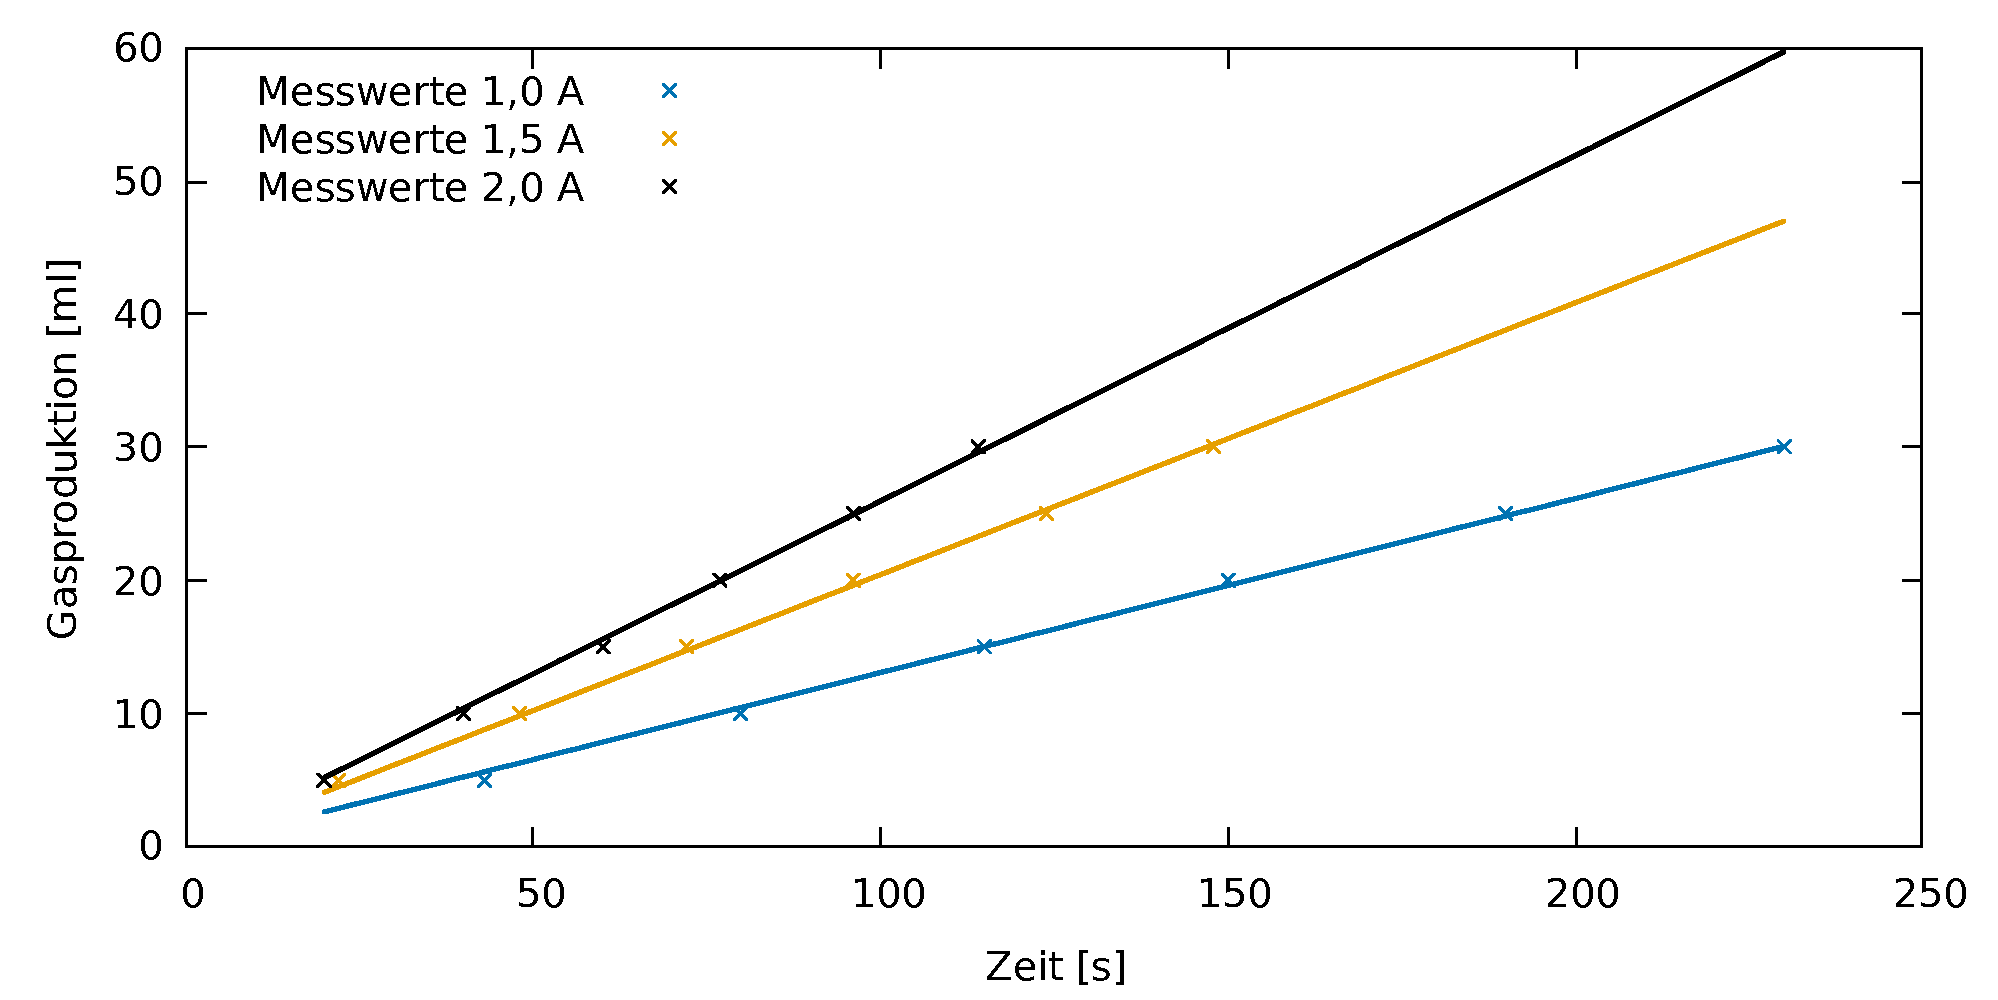
\includegraphics[width=0.8\textwidth]{mess/aufg8.pdf}
	\caption{Gasproduktion pro Zeit bei konstanter Last}
	\label{a8}
\end{figure}

\[ n=\frac{W_{HV}}{W_{el}} \]
\[
n(\SI{1}{\ampere})=0.95 \quad
n(\SI{2}{\ampere})=0.96 \quad
n(\SI{2,5}{\ampere})=0.92
\]
Diese Werte sind sehr gut. Eine gute Ausbeute bei der Aufspaltung von $H_2O$ ist wünschenswert.
Die Herstellung von Wasserstoff ist also sehr effizient ist. Das Gas nutzt man später für die Brennstoffzelle.

Im Graphen 3.7 zu sehen ist, wie viel Gas bei einer konstanten Stromlast hergestellt wird. Mit den theoretisch berechneten Werten der Gasentwicklung nach dem Faraday’schen Gesetz, ermittelt man den Faradayschen Wirkungsgrad und überprüft damit das Gesetz. Man erhält das Verhältnis von theoretisch errechneter zu tatsächlich erzeugter Gasmenge.
Hierzu nutzt man die Formeln:
$Q=nzF$
mit dem molaren Volumen $V_m=V_n=\SI{24,465}{\litre}$,
z ist 2, denn es werden beide H-Atome des $H_2O$ reduziert.
$I=\frac{VzF}{Vnt}$
$\frac{dV}{dt}=I \cdot \SI{0.127}{\centi \meter \cubed \per \ampere \second}$
Berechnen sich unsere Faraday’schen Wirkungsgrade auf:
\[
nF(\SI{1}{\ampere})=1,02 \quad nF(\SI{2}{\ampere}) = 1.05 \quad nF(\SI{2.5}{\ampere})=1.04
\]
Die Werte sind größer als eins, was auf manche Fehlerquellen verweisen muss. Da dieses Gesetz die chemischen Vorgänge beschreibt, sollte die Werte nahe der eins, aber keines Falls größer der eins, liegen.
Probleme stellten beispielsweise das Ablesen der Gasmenge dar.
Die angebrachte Skala war recht unhandlich und grob abzulesen.


\section{Brennstoffzelle}

Für die Brennstoffzolle soll nun die I/U-Kennlinie aufgenommen werden, hieraus lassen sich viele nützliche Daten, wie z.B. Leerlaufspannung, Kurzschlussstrom und Leistung, errechnen. Dazu wird der zwischengeschaltete Widerstand, von 0,5 Ohm bis mehrere hundert Kilo-Ohm, variiert. Verwendet wird hier das vorher hergestellte Wasserstoffgas.
\begin{figure}
	\centering
	\includegraphics[width=0.8\textwidth]{mess/aufg10.pdf}
	\caption{I/U-Kennlinie der Brennstoffzelle: durch den, auch ohne zusätzlich vorgeschaltetes Bauteil, hohen Widerstand des Aufbaus, ist die Kennlinie linear}
	\label{a10}
\end{figure}

Um den Maximum Power Point zu bestimmt nutzen wir die P/I Kennlinie. Unsere P/I Kurve bis zum Ende hin steigt, da kein geringerer Widerstand als $\SI{0,8}{\ohm}$  in den Stromkreis geschlossen werden konnte und der Kurzschlussstrom die Brennstoffzelle zerstören kann.
Wir benennen also unseren MPP an der Stelle von 0.8 Ohm und bekommen folgenden Wert: $P_{MPP} = \SI{95}{\milli \watt}$
Dieser Wert ist akzeptabel, aber nicht das Optimum der Brennstoffzelle.
\begin{figure}[htbp]
	\centering
	\includegraphics[width=0.8\textwidth]{mess/aufg11.pdf}
	\caption{P/I-Kennlinie der Brenstoffzelle: linearer Anstieg}
	\label{a11}
\end{figure}

Nun soll bei konstanter Last die verbrauchte Gasmenge bestimmt werden:
\begin{figure}[htbp]
	\centering
	\includegraphics[width=0.8\textwidth]{mess/aufg12.pdf}
	\caption{Gasdurchsatz der Brennstoffzelle bei konstanter Leistung}
	\label{a12}
\end{figure}
Wir bestimmen nun analog zum Elektrolyseur den elektrischen und Faraday’schen Wirkungsgrad der Brennstoffzelle.
Bei $\SI{0.13}{\volt}$ und $\SI{-128}{\milli \ampere}$ hat die Zelle am meisten Gas verbraucht uns somit am meisten Leistung gebracht. Es ergeben sich folgende Werte:
\begin{align*}
n_el &= \frac{W_{el}}{HHH2V}=0.39 \\
n_F &= \frac{V_{theo}}{V}=0.83
\end{align*}
Klar war für uns: Die Erzeugung von Strom durch den Verbrauch von Wasserstoff und Sauerstoff zu Wasser kann nicht perfekt Funktionieren.
Dennoch ist sie mit ca. 40\% keine schlechte Alternative zum Ottomotor.
Theoretisch sind wohl noch bessere Werte möglich, mit geringerem Widerstand und einer moderneren Vorrichtung.
